\documentclass[aspectratio=169, 10pt]{beamer}

% Theme and typography
\usetheme{Madrid}
\usecolortheme{whale}
\setbeamertemplate{navigation symbols}{}
\setbeamertemplate{caption}[numbered]

% Packages
\usepackage{amsmath, amssymb}
\usepackage{booktabs}
\usepackage{graphicx}
\usepackage{hyperref}
\usepackage{xcolor}

\definecolor{nflblue}{RGB}{1, 51, 105}
\definecolor{nflred}{RGB}{213, 10, 10}
\definecolor{darkslate}{RGB}{27, 38, 59}

\setbeamercolor{palette primary}{bg=nflblue, fg=white}
\setbeamercolor{palette secondary}{bg=darkslate, fg=white}
\setbeamercolor{palette tertiary}{bg=nflblue!80, fg=white}
\setbeamercolor{titlelike}{parent=palette primary}
\setbeamercolor{block title}{bg=nflblue, fg=white}
\setbeamercolor{block body}{bg=gray!10, fg=black}

\title[\textbf{Behind the Draft Board}]{\textbf{Beyond the Stopwatch, Behind the Draft Board:\\What Combine Tracking Adds Once Draft Position Is Known}}
\subtitle{NFL Big Data Bowl 2027 --- Analytics Track}
\author[M. Polley]{\textbf{Michael Polley}}
\institute[BDB 2027]{NFL Big Data Bowl 2027}
\date{\today}

\begin{document}

% 1
\begin{frame}
  \titlepage
\end{frame}

% 2
\begin{frame}{The Question That Matters on Draft Day}
  \begin{columns}[T]
    \begin{column}{0.5\textwidth}
      \begin{itemize}
        \item 10 Hz optical tracking records every Combine drill, not just the stopwatch time.
        \item Raw correlations look strong: receiver cut speed, lineman acceleration and DB break speed all track career snaps.
        \item But \textbf{teams play the players they drafted early}. Snaps follow draft capital.
        \item The useful question: does a metric predict playing time \textbf{beyond what the draft slot already predicts}?
      \end{itemize}
    \end{column}
    \begin{column}{0.5\textwidth}
      \begin{block}{\textbf{Answer}}
        \small
        \begin{itemize}
          \item All four headline metrics: significant alone ($p = 0.002$--$0.042$).
          \item All four after draft controls: \textbf{not significant} ($p = 0.32$--$0.80$).
          \item Draft slot explains \textbf{51\%} of WR snap variance; tracking adds \textbf{0.2 points}.
          \item Two per-snap efficiency leads at $p \approx 0.06$: test them on the 2026 class.
        \end{itemize}
      \end{block}
    \end{column}
  \end{columns}
\end{frame}

% 3
\begin{frame}{Data, Metrics and the Two Specifications}
  \begin{columns}[T]
    \begin{column}{0.52\textwidth}
      \small
      \textbf{Metrics (510 prospects, 2023--2025)}
      \begin{itemize}
        \item WR $s_{\text{cut}}$: median speed in curl, comeback, speed-out, slant.
        \item WR $z_{\text{cut}}$: per-drill median, z-scored \emph{within the drill}, averaged.
        \item DL / OL $\gamma_{\text{OE}}$: 90th-pct.\ $|a|$ residualised on weight.
        \item DB: 90th-pct.\ speed in the 45$^\circ$ transition drill.
      \end{itemize}
      \textbf{Outcomes}: career snaps, starter ($\ge 10$ starts), and regular-season per-snap efficiency (249,269 snaps).
    \end{column}
    \begin{column}{0.46\textwidth}
      \small
      \textbf{Raw}: $y = \beta_0 + \beta_1 m + \beta_2 c$\\[0.4em]
      \textbf{Controlled}: add $\log(\text{pick})$, UDFA flag, draft-class and position fixed effects.
      \vspace{0.6em}
      \begin{block}{\textbf{Two definition fixes}}
        \footnotesize
        \begin{itemize}
          \item Prospects ran different drills: Smith-Njigba's pooled median (24.0 km/h) is mostly gauntlet; his cutting median is 19.6.
          \item $a$ is a magnitude: $\gamma$ counts braking too, and pooled over drills it rises with drills run ($r = 0.36$).
        \end{itemize}
      \end{block}
    \end{column}
  \end{columns}
\end{frame}

% 4
\begin{frame}{Main Result: Every Effect Collapses Under Draft Controls}
  \begin{columns}[c]
    \begin{column}{0.58\textwidth}
      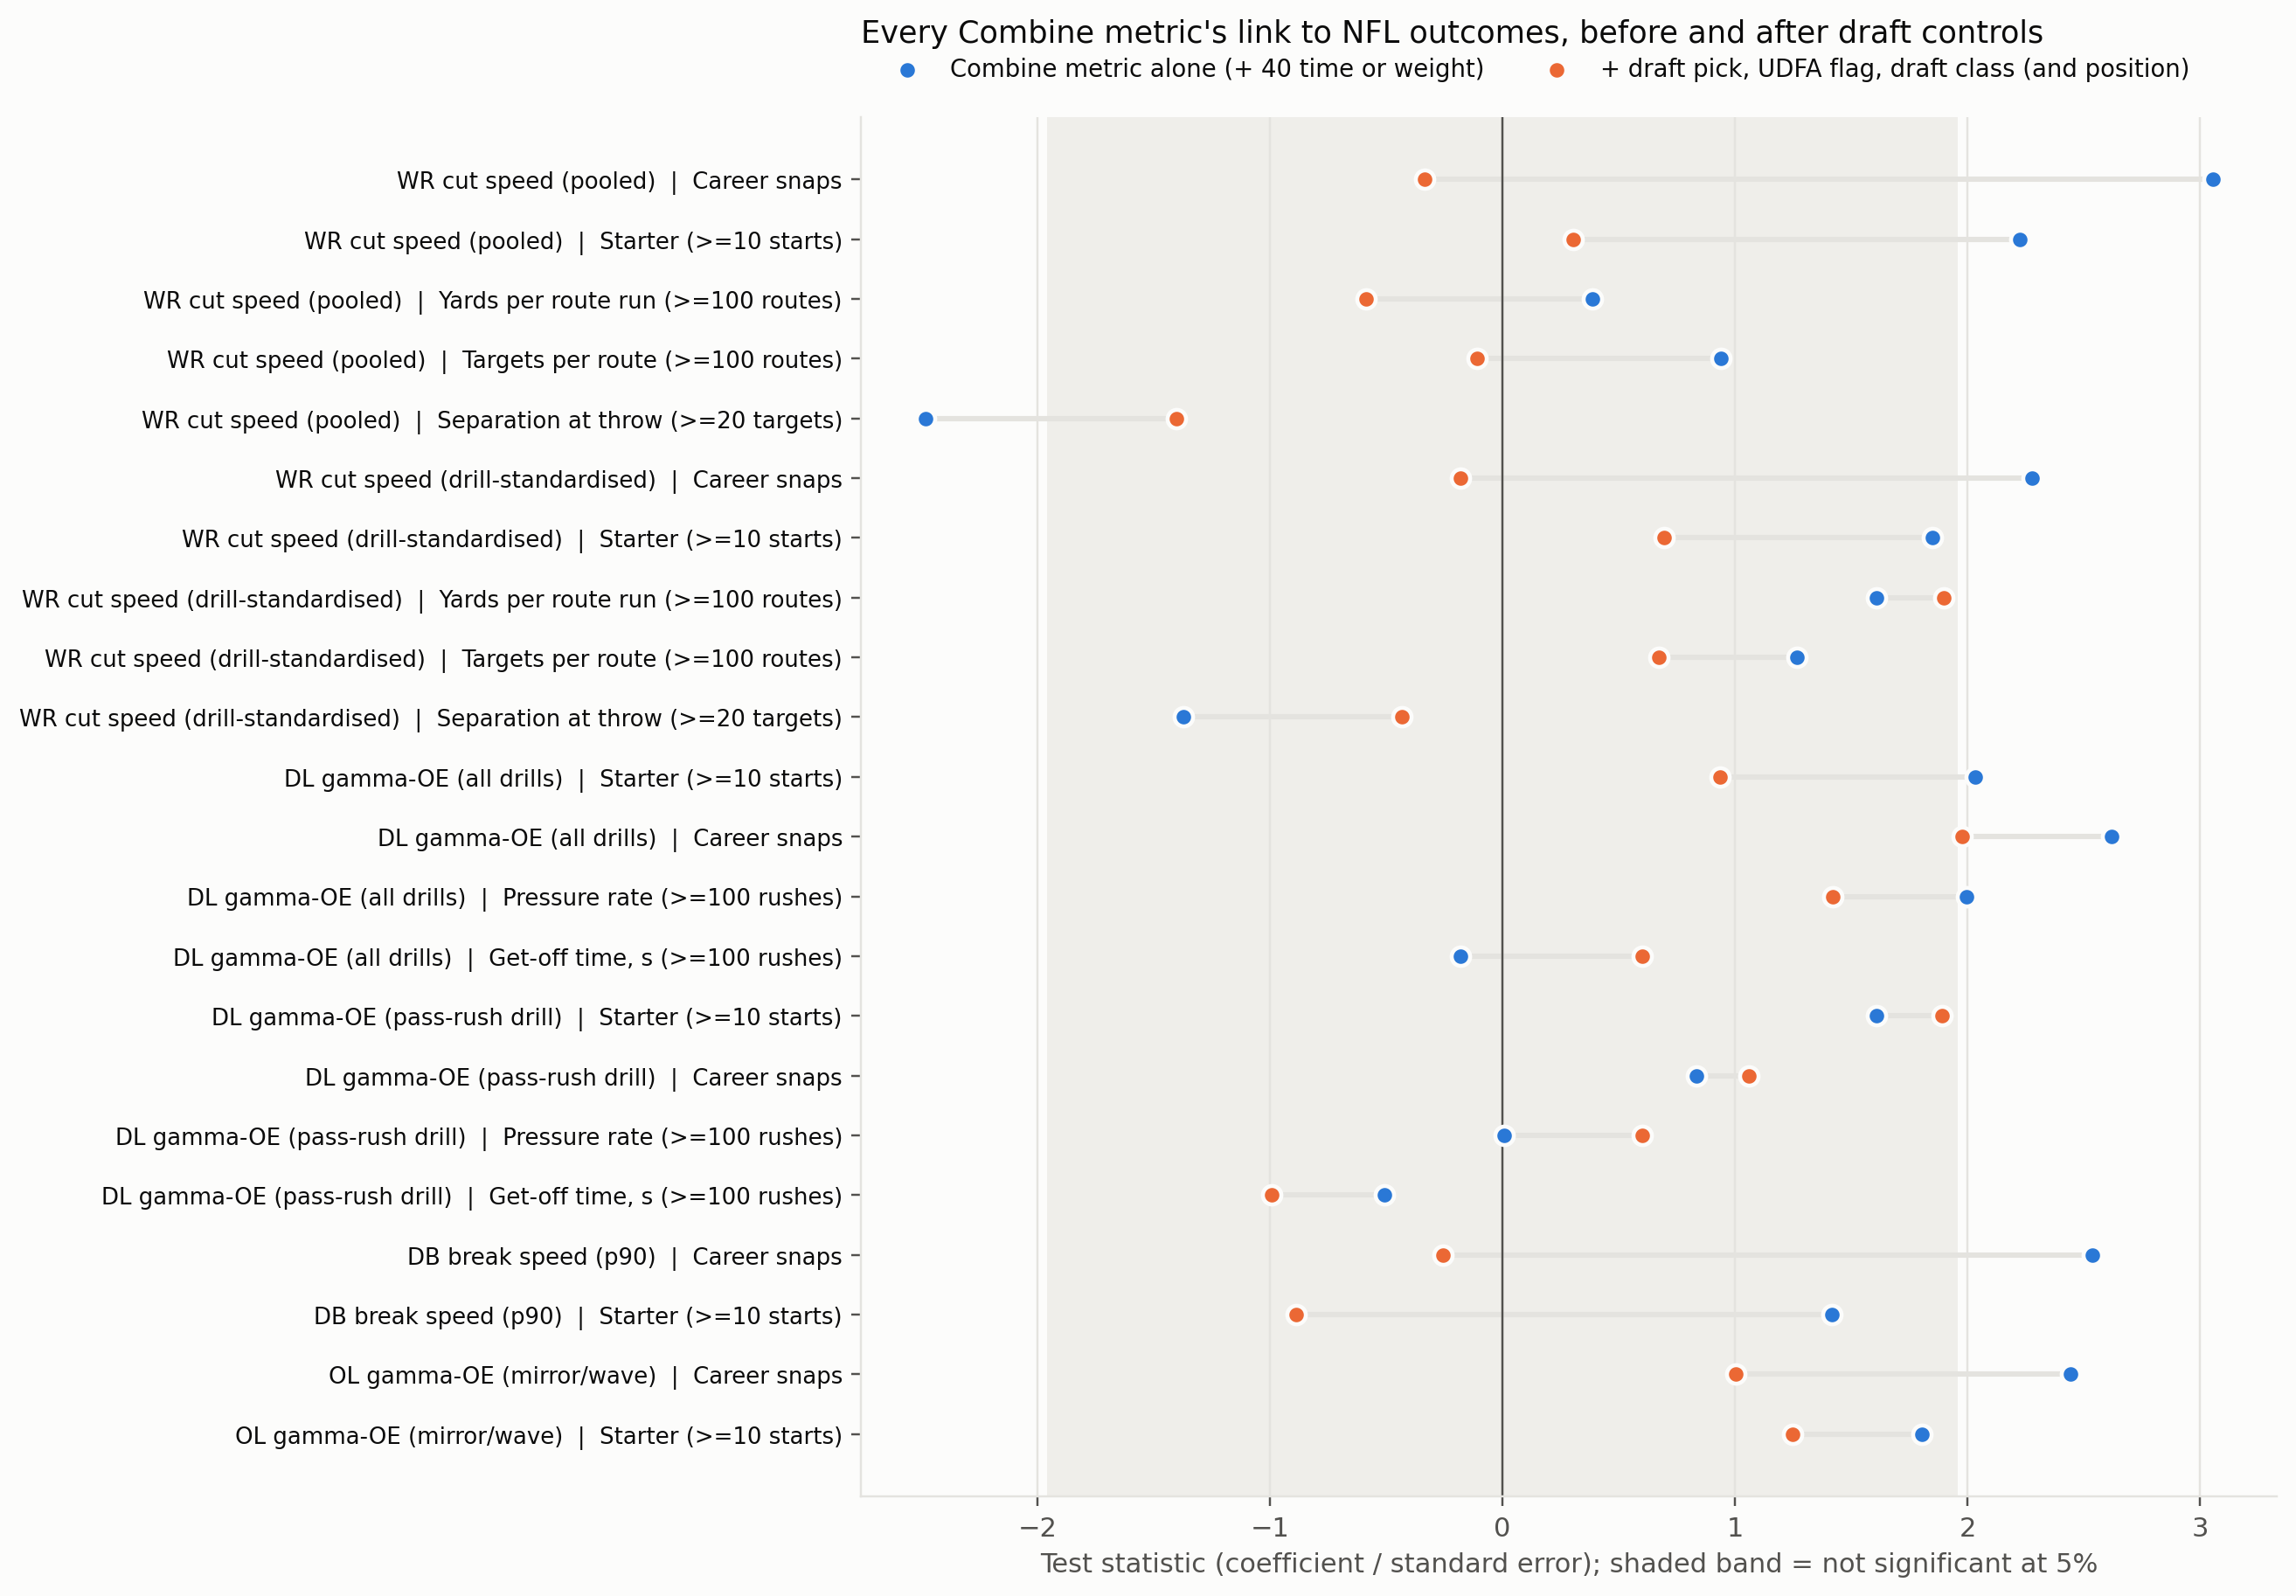
\includegraphics[width=\textwidth]{draft_controls.png}
    \end{column}
    \begin{column}{0.42\textwidth}
      \footnotesize
      \begin{tabular}{lcc}
        \toprule
        \textbf{Metric $\to$ outcome} & \textbf{Alone} & \textbf{+ Draft} \\
        \midrule
        WR $s_{\text{cut}}$ $\to$ snaps & $p{=}0.002$ & $p{=}0.74$ \\
        WR $s_{\text{cut}}$ $\to$ starter & $p{=}0.026$ & $p{=}0.76$ \\
        DL $\gamma_{\text{OE}}$ $\to$ starter & $p{=}0.042$ & $p{=}0.35$ \\
        DB break $\to$ snaps & $p{=}0.011$ & $p{=}0.80$ \\
        OL $\gamma_{\text{OE}}$ $\to$ snaps & $p{=}0.015$ & $p{=}0.32$ \\
        \bottomrule
      \end{tabular}
      \vspace{0.5em}
      \begin{itemize}
        \item 22 controlled tests; one at $p < 0.05$ (about one expected by chance).
        \item None survives Holm correction.
      \end{itemize}
    \end{column}
  \end{columns}
\end{frame}

% 5
\begin{frame}{Why: The Draft Board Already Prices Movement}
  \begin{table}
    \centering
    \small
    \begin{tabular}{lcccc}
      \toprule
      \textbf{WR tier (career starts)} & \textbf{N} & \textbf{Mean $s_{\text{cut}}$} & \textbf{Mean pick (UDFA = 262)} & \textbf{Undrafted} \\
      \midrule
      Top ($\ge 20$) & 14 & 18.03 km/h & 62 & 0\% \\
      Middle (3--19) & 40 & 17.19 km/h & 116 & 10\% \\
      Fringe ($\le 2$) & 52 & 16.53 km/h & 184 & 50\% \\
      \bottomrule
    \end{tabular}
  \end{table}
  \begin{itemize}
    \item Raw gap Top vs Fringe: Welch $t = 4.75$, $p < 0.001$, Cohen's $d = 1.00$.
    \item Faster cutters are drafted earlier (slope on $\log(\text{pick})$, $p = 0.012$).
    \item Snap $R^2$: draft variables $0.511$; draft + cut speed + 40 time $0.513$.
    \item \textbf{The gap is real, but scouts already see it.} It does not identify who outplays their slot.
  \end{itemize}
\end{frame}

% 6
\begin{frame}{What Is Left: Two Per-Snap Efficiency Leads}
  \begin{columns}[T]
    \begin{column}{0.5\textwidth}
      \begin{block}{\textbf{WR: $z_{\text{cut}}$ $\to$ yards per route run}}
        \small
        $+0.32$ YPRR per unit, $p = 0.058$, $N = 57$ (100+ routes), after draft controls.\\
        Pooled $s_{\text{cut}}$: nothing ($p = 0.56$). The drill fix exposes the lead.
      \end{block}
      \begin{block}{\textbf{DL: pass-rush-drill $\gamma_{\text{OE}}$ $\to$ starter}}
        \small
        Odds ratio $1.60$, $p = 0.059$, after draft and position controls.\\
        But flat on pressure rate ($p = 0.55$) and get-off ($p = 0.32$).
      \end{block}
    \end{column}
    \begin{column}{0.48\textwidth}
      \begin{block}{\textbf{No support for the separation story}}
        \small
        Separation at the throw does not rise with cut speed: raw slope $-0.08$ yd per km/h ($p = 0.013$), $p = 0.16$ with controls.
      \end{block}
      \vspace{0.4em}
      \small
      Both leads sit just above $p = 0.05$ in a family of 22 tests. They are hypotheses for a pre-registered test, not draft rules.
    \end{column}
  \end{columns}
\end{frame}

% 7
\begin{frame}{Case Study: Same Brake, Different Exit}
  \begin{center}
    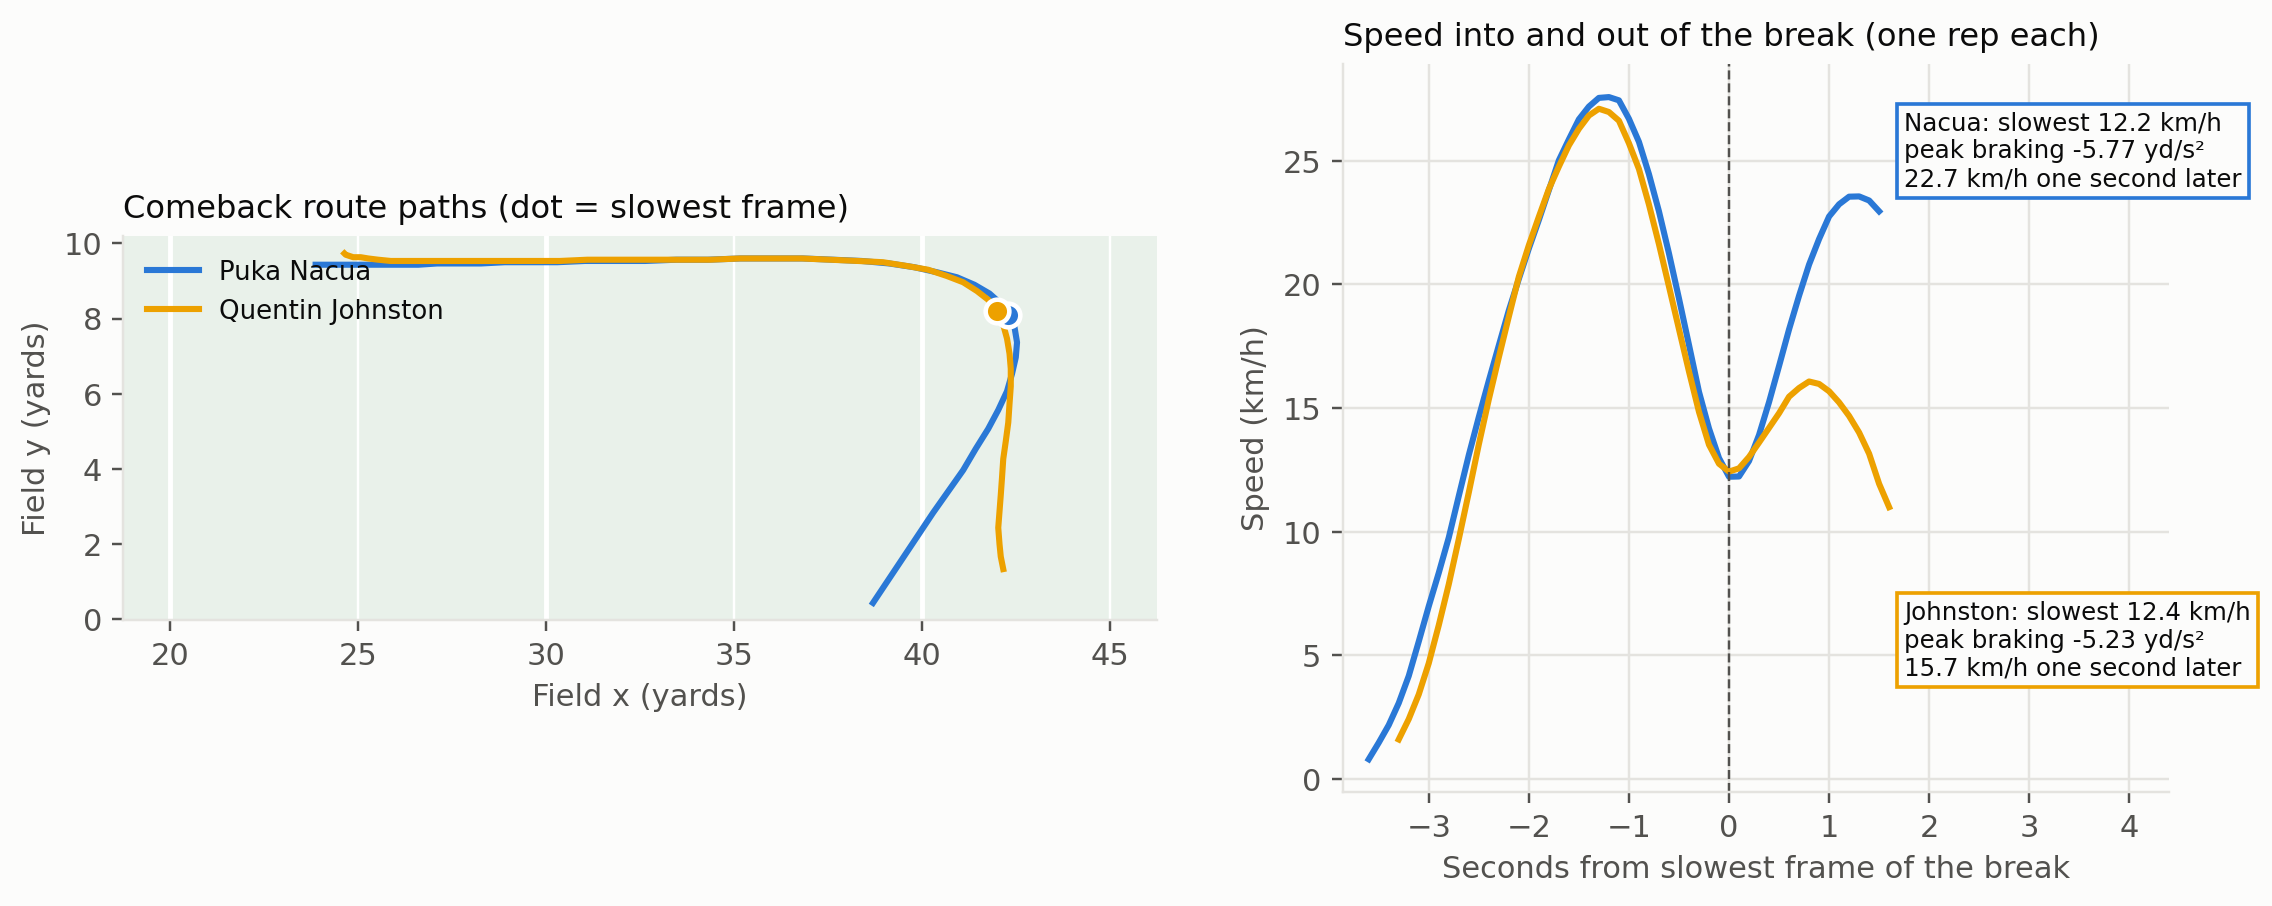
\includegraphics[width=0.9\textwidth]{route_kinematics_field_plot.png}
  \end{center}
  \vspace{-0.3cm}
  \small
  \begin{itemize}
    \item Nacua and Johnston enter the break alike (stem peak 27.6 / 27.1, slowest 12.2 / 12.4 km/h; each sheds $\approx$385--390 kg$\cdot$m/s).
    \item One second later: Nacua \textbf{22.7 km/h}, Johnston \textbf{15.7 km/h} and slowing. Re-acceleration is a candidate feature; one rep each is an anecdote.
  \end{itemize}
\end{frame}

% 8
\begin{frame}{Defensive Line: Mass-Adjusted Acceleration}
  \begin{columns}[c]
    \begin{column}{0.56\textwidth}
      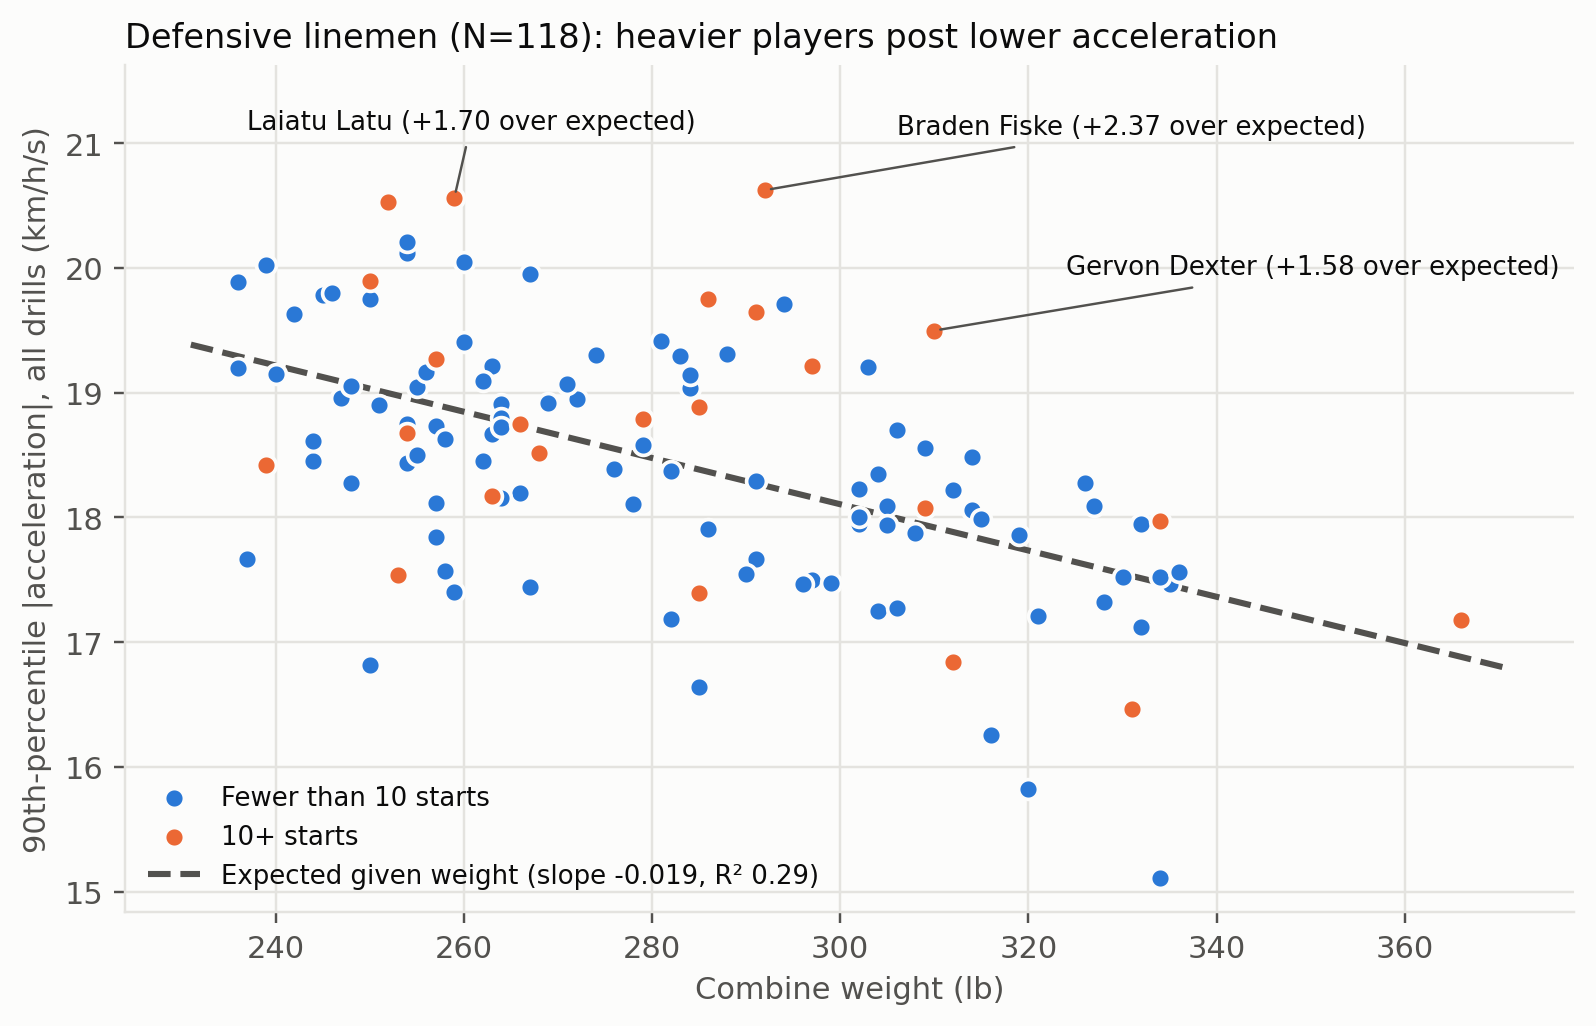
\includegraphics[width=\textwidth]{mass_vs_gamma_scatter.png}
    \end{column}
    \begin{column}{0.44\textwidth}
      \small
      \begin{itemize}
        \item Weight explains 29\% of $\gamma$ ($-0.019$ km/h/s per lb), so residualising is right.
        \item Fiske (+2.37), Latu (+1.70), Dexter (+1.58): all starters (24, 17, 33 starts).
        \item They were also picks 39, 15 and 53. Once pick is known, $\gamma_{\text{OE}}$ adds little: starter OR $1.85 \to 1.52$ ($p = 0.35$).
      \end{itemize}
    \end{column}
  \end{columns}
\end{frame}

% 9
\begin{frame}{Which Factors Predict Performance?}
  \footnotesize
  \resizebox{\textwidth}{!}{%
  \begin{tabular}{lllll}
    \toprule
    \textbf{Outcome} & \textbf{1st} & \textbf{2nd} & \textbf{3rd} & \textbf{Best tracking} \\
    \midrule
    WR starter (AUC) & Draft pick 0.87 & NGS final 0.78 & NGS college prod.\ 0.74 & Cut speed 0.69 \\
    DL starter (AUC) & Draft pick 0.82 & NGS final 0.76 & NGS college prod.\ 0.74 & Pass-rush $\gamma_{\text{OE}}$ 0.65 \\
    DB starter (AUC) & Draft pick 0.90 & NGS final 0.81 & NGS college prod.\ 0.76 & Break speed 0.63 \\
    OL starter (AUC) & Draft pick 0.93 & NGS final 0.86 & NGS college prod.\ 0.85 & $\gamma_{\text{OE}}$ 0.67 \\
    \midrule
    WR YPRR, beyond pick & \textbf{$z_{\text{cut}}$ +0.33} ($p{=}0.008$) & NGS college +0.21 & NGS athl.\ $-0.19$ & (1st) \\
    DL pressure, beyond pick + pos. & NGS final +0.36 ($p{=}0.003$) & \textbf{10-yd split $-0.29$} ($p{=}0.034$) & Bench +0.29 ($N{=}34$) & $\gamma_{\text{OE}}$ +0.24 \\
    \bottomrule
  \end{tabular}}
  \vspace{0.6em}
  \small
  \begin{itemize}
    \item \textbf{Playing time:} draft pick first everywhere; no predictor adds more than 0.01 AUC on top of it.
    \item \textbf{Efficiency:} Combine information shows up here. For pass rushers, \textbf{faster 10-yard split and 40 time go with more pressure} at the same pick and position.
    \item Exploratory: 7 of 30 efficiency correlations below $p = 0.05$ (1.5 expected); none survives Holm.
  \end{itemize}
\end{frame}

% 10
\begin{frame}{Guidance for Front Offices}
  \small
  \begin{enumerate}
    \item \textbf{Test conditional on draft slot.} A raw link to snaps or starts mostly restates the draft board.
    \item \textbf{Standardise within each drill.} Prospects run different drill sets; pooled medians mix them.
    \item \textbf{Judge on per-snap efficiency}, not snap volume.
    \item \textbf{Keep the stopwatch for pass rushers.} Short-area speed relates to pressure rate beyond draft slot.
    \item \textbf{Pre-register the leads on the 2026 class:} $z_{\text{cut}} \to$ YPRR; 10-yard split $\to$ pressure rate; pass-rush $\gamma_{\text{OE}} \to$ starter.
  \end{enumerate}
  \footnotesize
  \textbf{Limitations:} 1--3 seasons of careers; small efficiency samples (57 receivers, 69 rushers); one tracked rep per drill; $a$ cannot separate acceleration from braking.
  Every number is printed by the scripts in \texttt{scripts/}; results in \texttt{results/}.
  \vspace{0.3em}
  \begin{center}
    \textbf{Thank you. Questions and discussion.}
  \end{center}
\end{frame}

\end{document}
